\documentclass[crop,convert=pdf2svg]{standalone}

\usepackage{tikz}
\usetikzlibrary{arrows, calc, fit}
\begin{document}

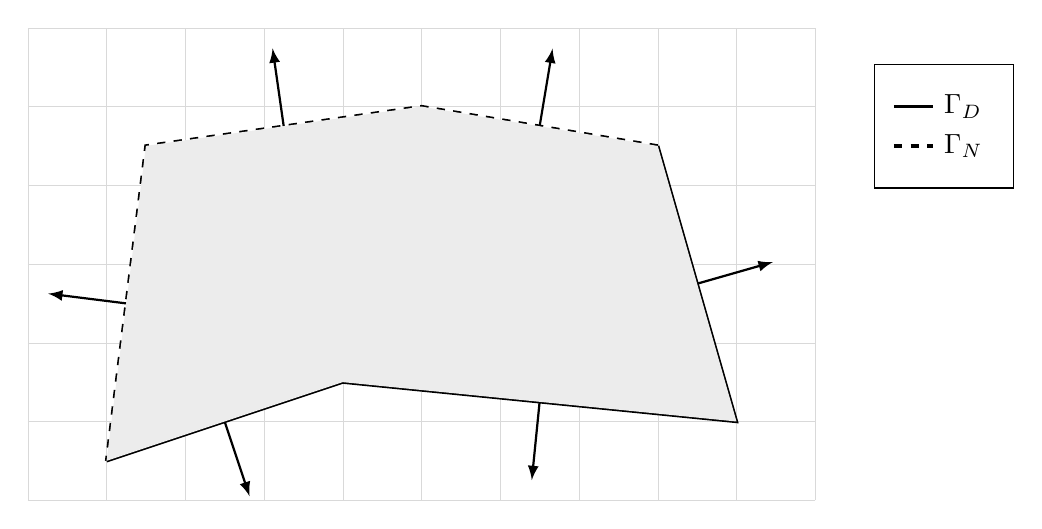
\begin{tikzpicture}[>=latex]
  \draw[line width=0.1pt,gray!30] (0,0) grid (10,6); 
  \draw[fill=none] (1,0.5) coordinate(a);
  \draw[fill=none] (4,1.5)  coordinate(b);
  \draw[fill=none] (9,1)  coordinate(c);
  \draw[fill=none] (8,4.5)  coordinate(d);
  \draw[fill=none] (5,5)  coordinate(e);
  \draw[fill=none] (1.5,4.5)  coordinate(f);
  \draw[very thick] (a) -- (b) -- (c) -- (d);
  \draw[very thick, dashed] (d) --(e) --(f) -- (a);
  %($(A)!0.5!90:(B)$)
  \coordinate (af) at ($(a)!0.5!(f)$);
  \draw [-latex, thick] (af) -- ($(af)!1cm!90:(f)$); 
  \coordinate (ba) at ($(b)!0.5!(a)$);
  \draw [-latex, thick] (ba) -- ($(ba)!1cm!90:(a)$); 
  \coordinate (cb) at ($(c)!0.5!(b)$);
  \draw [-latex, thick] (cb) -- ($(cb)!1cm!90:(b)$); 
  \coordinate (dc) at ($(d)!0.5!(c)$);
  \draw [-latex, thick] (dc) -- ($(dc)!1cm!90:(c)$); 
  \coordinate (ed) at ($(e)!0.5!(d)$);
  \draw [-latex, thick] (ed) -- ($(ed)!1cm!90:(d)$); 
  \coordinate (fe) at ($(f)!0.5!(e)$);
  \draw [-latex, thick] (fe) -- ($(fe)!1cm!90:(e)$); 
  \path [fill=gray!15]  (a) -- (b) -- (c) -- (d)--(e) --(f) -- (a);

  \coordinate (gd0) at (11,5);
  \coordinate (gn0) at (11,4.5);
  \draw[very thick] (gd0) -- (11.5,5) node[right] (gD) {$\Gamma_D$};
  \draw[very thick, dashed] (gn0) -- (11.5,4.5) node[right] (gN){$\Gamma_N$};

  \node[fit=(gd0)(gn0)(gD)(gN),draw,inner sep=0.25cm] (Box) {};
  \end{tikzpicture}
\end{document}